\section{Commande de base pour \mbpy}

%   logo mb dans la table des matières
\logo{mbpy}

% style de page micro:bit
\pagestyle{mbpy}

\subsection{Description}

\subsubsection{Objectif}

\begin{formule}
Il est possible de programmer la carte \mb avec Python. Pour cela, il faut utiliser le module \mb.

Dans cette fiche, vous découvrirez les commandes essentielles de ce module.
\end{formule}


\subsubsection{Matériel}
\begin{itemize}
    \item 1 $\times$ \matosMb
    \item 1 $\times$ IDE programmation python (Mu) : à télécharger/installer en \href{cliquant ici}{https://codewith.mu/}
\end{itemize}




\subsection{Commandes essentielles}

%
% activité de niveau 1
%
% commande perso \CARTOUCHE
%   5 paramètres : 
%       * durée
%       * public
%       * travail en maths
%       * travail en sciences
%       * travail en algo
\cartouche{2 h}{2de}{}{}{affichage ; bouton ; événement.}


\subsubsection{Le module \pyline{microbit}}

En Python, les entrées/sorties de la carte \mb ne sont pas \textit{nativement} accessibles. Afin de pouvoir utiliser les fonctions prévues à cet effet, il faut appeler le module \pyline{microbit}.\par
Pour appeler ce module, il faut utiliser la commande classique \pyline{from ... import ...}
    
    
\begin{methode}
\pyfile{1}{1}{./res/mbpy-initiationPython.py.tex}
\end{methode}

\begin{astuce}
La bibliothèqe \pyline{microbit} est déjà téléchargée et préinstallée avec le logiciel \texttt{mu-editor}. Mais il faut tout de même l'appeler pour l'utiliser
\end{astuce}

Le module \pyline{micropython} introduit des \textbf{classes} (avec \emph{instances}, \emph{méthodes} et \emph{propriétés}) et des \textbf{modules} (avec \emph{fonctions} et  \emph{constantes}).

\begin{minipage}[t]{0.5\linewidth}
    Exemple de classes :
    \begin{description}
        \item[Image] pour créer et manipuler les images. Les \emph{propriétés} sont des images déjà enregistrées (comme les smileys)
        \item[Button] avec deux \emph{instances} \texttt{button\_a} et \texttt{button\_b} pour connaître l'état des boutons. 
        \item[\textit{Pin}] avec différentes \emph{instances} en fonction du type de broche (digitale, analogique ou de contact comme \texttt{pin0},  \texttt{pin1} et  \texttt{pin2}).
    \end{description}
\end{minipage}
%
\begin{minipage}[t]{0.5\linewidth}
    Exemple de modules :
    \begin{description}
        \item[display] pour gérer l'écran de LED
        \item[accelerometer] pour interroger l'accéléromètre
        \item[compass] pour manipuler et interroger la boussole
        \item[music] pour créer et manipuler de la musique
        \item[speech] pour faire parler le \mb
        \item[radio] pour communiquer entre \mb via un protocole simple
    \end{description}
\end{minipage}

\begin{remarque}
\textbf{Pour aller plus loin}, vous pouvez consulter la page  \href{https://microbit-micropython.readthedocs.io/fr/latest/microbit.html}{Microbit Module} de la documentation officielle.
\end{remarque}


\subsubsection{Micropython dans la carte \mb}

Lorsque la carte \mb est flashée avec le module \pyline{microbit}, elle contient un noyau micropython et peut donc exécuter du code python.

L'IDE \texttt{Mu} permet d'accéder au noyau micropython de la carte. Pour \textbf{accéder au terminal} de ce noyau, il suffit de cliquer sur l'icône REPL de l'application.

Il est alors tout à fait possible d'écrire du code dans ce terminal qui sera exécuté par la carte \mb.

\begin{remarque}
    L'instruction \pyline{print()} permet d'écrire dans le terminal REPL.
\end{remarque}

\begin{methode}
Pour utiliser le terminal de la carte \mb :
\begin{itemize}
    \item Flasher la carte \mb avec micropython.
    \item Ouvrir le terminal de la carte en cliquant sur REPL
    \item saisir le code ci-dessous :\\
\begin{minted}[bgcolor=grisClair]{console}
> print("Hello, World!")
\end{minted}
\end{itemize}
\end{methode}

\begin{methode}
    Le programme ci-dessous affiche 10 fois le même texte dans le terminal :
    \pyfile{238}{240}{./res/mbpy-initiationPython.py.tex}
\end{methode}


\subsubsection{Afficher un texte}

Le module \pyline{display} permet de gérer l'écran de LED de \mb.\par
La fonction \pyline{display.show("string")} permet d'\emph{afficher} un texte.\\
La fonction \pyline{display.scroll("string")} permet de le faire \emph{défiler}.

\begin{methode}
\pyfile{4}{6}{./res/mbpy-initiationPython.py.tex}
\end{methode}

\begin{remarque}
\textbf{Pour aller plus loin}, vous pouvez consulter les pages \href{https://microbit-micropython.readthedocs.io/fr/latest/tutorials/hello.html}{Introduction >> Hello, World!} et \href{https://microbit-micropython.readthedocs.io/fr/latest/display.html}{Display} de la documentation officielle.
\end{remarque}


\subsubsection{Des images}

La classe \pyline{Image} contient comme \emph{propriétés} de nombreuses images pré-programmées. Par exemple l'image du coeur : \pyline{Image.HEART}

\begin{center}
    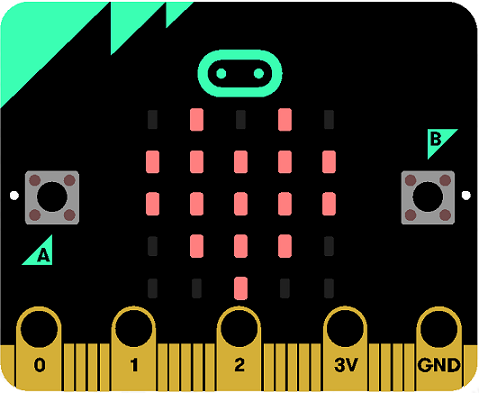
\includegraphics[width=3cm]{res/mbpy-init-heart.png}
\end{center}

Pour afficher une image, il faut utiliser la fonction \pyline{display.show()}.
La fonction \pyline{display.clear()} permet d'effacer l'écran.

Pour afficher successivement des images, il faut mettre le \mb en pause. Sinon l'utilisateur n'aura pas le temps de tout voir. La commande \pyline{sleep(nombreEntier)} arrête donc la carte pendant la durée (en milliseconde) indiquée.

\begin{methode}
Le code Python ci-dessous affiche une image pendant une seconde puis affiche une deuxième image. Une seconde plus tard, l'écran s'efface.

\pyfile{22}{27}{./res/mbpy-initiationPython.py.tex}
\end{methode}

\begin{remarque}
\textbf{Pour aller plus loin}, vous pouvez consulter les pages  \href{https://microbit-micropython.readthedocs.io/fr/latest/tutorials/images.html}{Introduction >> Images} ou \href{https://microbit-micropython.readthedocs.io/fr/latest/image.html}{Image} de la documentation officielle.
\end{remarque}


\subsubsection{Des animations}

Lorsque plusieurs images sont stockées dans un \textbf{tableau}, il est possible de les faire défiler à un rythme donné. Ceci permet de facilement créer une \emph{animation}. 

Pour faire défiler des images, utiliser l'option \pyline{delay=nombreEntier}
de la fonction \pyline{display.show()}.

Le module \pyline{microbit} contient \textbf{deux} tableaux d'images :
\begin{itemize}
    \item \pyline{Image.ALL_CLOCKS} qui affiche la grande \emph{aiguille d'une montre} sous différentes orientations
    \item \pyline{Image.ALL_ARROWS} qui affiche des \emph{flèches} dans toutes les directions. 
\end{itemize}

\begin{methode}
Le code ci-dessous affiche toutes les 0,200 secondes l'aiguille d'une montre qui tourne :\par
\pyfile{42}{43}{./res/mbpy-initiationPython.py.tex}
\end{methode}

\begin{remarque}
\textbf{Pour aller plus loin}, vous pouvez consulter la page  \href{https://microbit-micropython.readthedocs.io/fr/latest/tutorials/images.html}{Introduction >> Images} de la documentation officielle.
\end{remarque}


\subsubsection{Des boutons}

Les états des boutons de la carte \mb sont récupérables par le module \pyline{micropython}. Il existe pour cela deux classes : \pyline{button_a} et \pyline{button_b}.

Ces deux classes possèdent 3 méthodes :
\begin{itemize}
    \item \pyline{.get_presses()} retourne le \textbf{nombre} de fois que le bouton a été pressé depuis le dernier appel de cette méthode
    \item \pyline{.is_pressed()} retourne un \textbf{booléen} qui indique si le bouton est \emph{actuellement} pressé
    \item \pyline{.was_pressed()} retourne un \textbf{booléen} qui indique si le bouton \emph{a été} pressé depuis le dernier appel de cette méthode.
\end{itemize}

\begin{methode}
Le code ci-dessous affiche le nombre de fois que le bouton A a été pressé depuis le démarrage.
\pyfile{89}{91}{./res/mbpy-initiationPython.py.tex}
\end{methode}

Pour programmer un \mb, il est très souvent nécessaire de détecter un \textbf{évènement} comme par exemple l'appui sur un bouton.\par
Une méthode simple consiste à créer une \textbf{boucle infinie} \pyline{while True:} contenant un test qui, à chaque itération de la boucle, vérifie la réalisation de l'évènement attendu.\par
Lorsque l'événement se réalise, l'instruction \pyline{break} est appelée pour sortir de la boucle.

\begin{methode}
Le code ci-dessous tourne en boucle.
\begin{itemize}
    \item Lorsque aucun évènement n'est détecté, c'est l'image triste \pyline{Image.SAD} qui s'affiche.
    \item Pendant que le bouton A est pressé, l'image joyeuse \pyline{Image.HAPPY} s'affiche.
    \item Pendant que la broche \pyline{pin1} est touchée (en même temps que la broche \texttt{GND}), l'image endormie \pyline{Image.ASLEEP} s'affiche.
    \item Lorsque le bouton B est pressé, l'écran s'efface et le programme quitte la boucle.
\end{itemize}

\pyfile{95}{105}{./res/mbpy-initiationPython.py.tex}
\end{methode}

\begin{remarque}
    Les broches instanciées \pyline{pin0}, \pyline{pin1} et \pyline{pin2} peuvent aussi servir de bouton. La méthode \pyline{.is_touched()} permet de renvoyer un booléen qui devient vrai lorsqu'une personne en contact avec la masse (broche \texttt{GND}) touche puis relâche la broche en question.
    
    En effet, lorsqu'une instance de ces broches est activée, la carte \mb mesure la résistance entre cette broche et la masse (broche \texttt{GND}). Lorsque cette dernière varie et passe d'une valeur quasi infinie à une valeur faible, le test devient vrai. Cet évènement arrive lorsqu'une personne en contact avec \texttt{GND} touche la broche et la relâche.
\end{remarque}

\begin{remarque}
\textbf{Pour aller plus loin}, vous pouvez consulter les pages  \href{https://microbit-micropython.readthedocs.io/fr/latest/tutorials/buttons.html}{Introduction >> Boutons} et \href{https://microbit-micropython.readthedocs.io/fr/latest/button.html}{Buttons} de la documentation officielle.
\end{remarque}


\subsubsection{Le hasard}

Le module \pyline{random} est utilisable avec \mb. Une fois \emph{importé}, il est très simple de générer des nombres aléatoires avec les fonctions \pyline{random.random()} ou \pyline{random.randint(a,b)}.

\begin{methode}
Le programme ci-dessous affiche très rapidement 50 nombres aléatoires tirés entre 1 et 6. Le dernier nombre tiré est affiché pendant une seconde puis effacé.
\pyfile{122}{128}{./res/mbpy-initiationPython.py.tex}
\end{methode}

\begin{remarque}
\textbf{Pour aller plus loin}, vous pouvez consulter les pages  \href{https://microbit-micropython.readthedocs.io/fr/latest/tutorials/random.html}{Introduction >> Hasard} et \href{https://microbit-micropython.readthedocs.io/fr/latest/random.html}{Random Number Generation} de la documentation officielle.
\end{remarque}


\subsubsection{Le mouvement}

L'accéléromètre du \mb est accessible par le module \pyline{accelerometer}.\\
Il est alors possible de récupérer une des coordonnées du vecteur accélération (avec une fonction du type \pyline{accelerometer.get_x()}.

\begin{methode}
Le programme ci-dessous affcihe une flèche en fonction de l'inclinaison du \mb.\\
Le bouton B permet de quitter cette boucle.

\pyfile{132}{144}{./res/mbpy-initiationPython.py.tex}
\end{methode}

\begin{remarque}
\textbf{Pour aller plus loin}, vous pouvez consulter les pages  \href{https://microbit-micropython.readthedocs.io/fr/latest/tutorials/movement.html}{Introduction >> Mouvement} et \href{https://microbit-micropython.readthedocs.io/fr/latest/accelerometer.html}{Accelerometer} de la documentation officielle.
\end{remarque}


\subsubsection{Les gestes}

Le module \pyline{accelerometer} peut aussi détecter des mouvements ou des positions pré-programmés : les \emph{gestes} (\texttt{"up"}, \texttt{"down"}, \texttt{"left"}, \texttt{"right"}, \texttt{"face up"}, \texttt{"face down"}, \texttt{"freefall"}, \texttt{"3g"}, \texttt{"6g"}, \texttt{"8g"}, \texttt{"shake"}).

Il y a alors 3 fonctions qui s'applique sur le module \pyline{accelerometer} :
\begin{itemize}
    \item \pyline{accelerometer.get_gestures()} retourne un \textbf{tuple} contenant l'historique des gestes. Le dernier élément du tuple est le geste le plus récent.Le tuple est réinitialisé à chaque appel de cette fonction.
    \item \pyline{accelerometer.is_gesture("nom")} retourne un \textbf{booléen} qui indique si le geste en cours est \pyline{"nom"}.
    \item \pyline{accelerometer.was_pressed("nom")} retourne un \textbf{booléen} qui indique si le geste \pyline{"nom"} \emph{a été} pressé depuis le dernier appel de cette fonction.
\end{itemize}

\begin{methode}
Le programme ci-dessous affiche le nombre "8"\\
Lorsque le \mb est secoué, il s'affiche une seconde plus tard de manière aléatoire et équiprobable soit "Oui", soit "Non".\\
Le jeu recommence sauf si on appui sur le bouton B ce qui fait sortir de la boucle.

\pyfile{163}{173}{./res/mbpy-initiationPython.py.tex}
\end{methode}

\begin{remarque}
\textbf{Pour aller plus loin}, vous pouvez consulter les pages  \href{https://microbit-micropython.readthedocs.io/fr/latest/tutorials/gestures.html}{Introduction >> Gestes} et \href{https://microbit-micropython.readthedocs.io/fr/latest/accelerometer.html}{Accelerometer} de la documentation officielle.
\end{remarque}


\subsubsection{La radio}

Les cartes \mb peuvent communiquer entres elles au moyen du module \pyline{radio}.

La fonction \pyline{radio.send("string")} permet d'envoyer par radio le texte \pyline{"string"}.

La fonction \pyline{radio.receive()} retourne la chaîne de caractère des données reçus par radio. Si rien n'a été reçu, la chaine vaut \pyline{None}

\begin{methode}
Le programme est à téléverser sur 2 cartes \mb. Un appui sur les boutons A ou B de l'un des \mb affiche les texte "A" ou "B" sur l'autre.

\pyfile{213}{215}{./res/mbpy-initiationPython.py.tex}\\
\pyfile{216}{217}{./res/mbpy-initiationPython.py.tex}\\
\pyfile{218}{223}{./res/mbpy-initiationPython.py.tex}\\
\pyfile{224}{229}{./res/mbpy-initiationPython.py.tex}\\
\pyfile{230}{234}{./res/mbpy-initiationPython.py.tex}
\end{methode}

\begin{remarque}
\textbf{Pour aller plus loin}, vous pouvez consulter les pages  \href{https://microbit-micropython.readthedocs.io/fr/latest/tutorials/radio.html}{Introduction >> Radio} et \href{https://microbit-micropython.readthedocs.io/fr/latest/radio.html}{Radio} de la documentation officielle.
\end{remarque}


\subsubsection{La boussole}

Pour interroger la boussole du \mb, il faut utiliser le module \pyline{compass}.\par 
Certaines fonctions comme \pyline{microbit.compass.get_x()} renvoient une composante du vecteur champ magnétique.\par 
La fonction\pyline{microbit.compass.heading()} renvoie l'angle en degré entre l'orientation de la carte \mb et le nord magnétique.

\begin{remarque}
    Avant d'utiliser une fonction du module \pyline{compass}, il faut obligatoirement \emph{calibrer} \mb.
    
    Pour cela, il est automatiquement demandé à l'utilisateur de bouger la carte dans différentes positions. Il faut que le point rouge qui clignote passe par toutes les LED de l'écran.
    
    Pour programmer une calibration de la carte, il est possible d'utiliser la commande \pyline{compass.calibrate()}.
\end{remarque}


\begin{methode}
Le programme ci-dessous fait office de boussole et indique le nord magnétique.

Attention, le capteur est sensible aux objets tels que téléphones, ordinateurs ou aux lieux tels que ascenseurs ou salle informatique\ldots

\pyfile{177}{185}{./res/mbpy-initiationPython.py.tex}
\end{methode}

\begin{remarque}
\textbf{Pour aller plus loin}, vous pouvez consulter les pages  \href{https://microbit-micropython.readthedocs.io/fr/latest/tutorials/direction.html}{Introduction >> Direction} et \href{https://microbit-micropython.readthedocs.io/fr/latest/compass.html}{Compass} de la documentation officielle.
\end{remarque}





\newpage

\subsection{Des commandes pour aller plus loin}
\cartouche{2 h}{2de}{}{}{affichage ; bouton ; événement ; son}


\subsubsection{Représentation graphique avec \texttt{Mu}}

Il est possible de tracer un \textbf{nuage de points} avec l'IDE \texttt{Mu}.

Pour cela, il faut 
\begin{itemize}
    \item utiliser l'outil \texttt{Graphique} de l'IDE \texttt{Mu},
    \item faire afficher par le programme en cours d'exécution un tuple de nombres.
\end{itemize}


\begin{methode}
Le programme ci-dessous affiche dans le terminal (ou \textbf{dans le Graphique} si l'outil de l'IDE est cliqué) des fréquences d'apparitions lors d'une expérience aléatoire.
\pyfile{244}{258}{./res/mbpy-initiationPython.py.tex}
\end{methode}



\subsubsection{Des images personnalisées}

Les images sont des objets qui peuvent être créées grâce au constructeur \pyline{Image("string")}.\par
Le texte \pyline{"string"} permet de décrire, \textbf{ligne par ligne}, la luminosité de chaque pixel de l'écran de LED. Pour chaque diode, la valeur varie de 0 (éteinte) à 9 (luminosité maximale). Pour séparer les lignes, il faut utiliser le symbole \pyline{":"}

\begin{methode}
Voici une image représentant un bateau avec la coque plus foncée que les 2 mâts :
\pyfile{31}{38}{./res/mbpy-initiationPython.py.tex}
\end{methode}

\begin{remarque}
\textbf{Pour aller plus loin}, vous pouvez consulter les pages  \href{https://microbit-micropython.readthedocs.io/fr/latest/tutorials/images.html}{Introduction >> Images} ou \href{https://microbit-micropython.readthedocs.io/fr/latest/image.html}{Image} de la documentation officielle.
\end{remarque}


\subsubsection{Des animations personnalisées}

En stockant des images personnalisées dans un tableau, il est possible de créer des \emph{animations personnalisées}.

\begin{methode}
Créer un image représentant un tableau et stocker cette image dans la variable \pyline{bateau1} :
\pyfile{47}{52}{./res/mbpy-initiationPython.py.tex}

Créer d'autres images (donnant l'illusion que le bateau s'enfonce) et les stocker dans de nouvelles variables:
\pyfile{54}{58}{./res/mbpy-initiationPython.py.tex}\\
\pyfile{60}{64}{./res/mbpy-initiationPython.py.tex}\\
\pyfile{66}{70}{./res/mbpy-initiationPython.py.tex}\\
\pyfile{72}{76}{./res/mbpy-initiationPython.py.tex}\\
\pyfile{78}{82}{./res/mbpy-initiationPython.py.tex}

Créer un tableau regroupant toutes les images et afficher l'animation :
\pyfile{84}{85}{./res/mbpy-initiationPython.py.tex}
\end{methode}

\begin{remarque}
\textbf{Pour aller plus loin}, vous pouvez consulter la page  \href{https://microbit-micropython.readthedocs.io/fr/latest/tutorials/images.html}{Introduction >> Images} de la documentation officielle.
\end{remarque}


\subsubsection{Faire parler \mb}

La carte \mb peut aussi \textbf{parler}.
Avant cela, il faut connecter un casque audio ou un (petit) haut-parleur à la carte.

\begin{center}
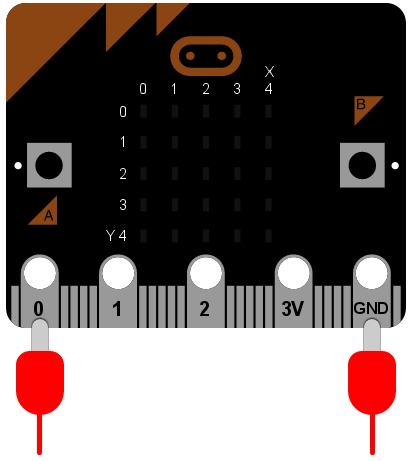
\includegraphics[width=3cm]{res/mbpy-init-audio.png}    
\end{center}

Le module \pyline{speech} contient les fonctions permettant de gérer la \emph{voix} de \mb, dont la fonction \pyline{speech.say("string")} qui fera parler.

\begin{methode}
\pyfile{16}{18}{./res/mbpy-initiationPython.py.tex}
\end{methode}

\begin{remarque}
\textbf{Pour aller plus loin}, vous pouvez consulter les pages  \href{https://microbit-micropython.readthedocs.io/fr/latest/tutorials/speech.html}{Introduction >> Speech} ou \href{https://microbit-micropython.readthedocs.io/fr/latest/speech.html}{Speech} de la documentation officielle.
\end{remarque}


\subsubsection{De la musique}

La carte \mb est capable de jouer de la musique. Pour cela, il faut au préalable \textbf{connecter un casque audio} ou un petit haut-parleur à la carte.

\begin{center}
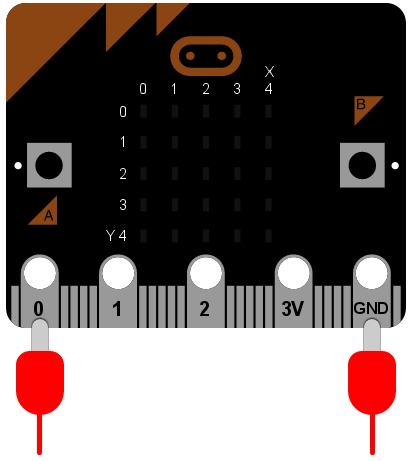
\includegraphics[width=3cm]{res/mbpy-init-audio.png}    
\end{center}

Le module \pyline{music} contient les fonctions permettant de gérer et de contrôler le son. Parmi elles, la fonction \pyline{music.play()} joue une mélodie.

Par ailleurs, le module  \pyline{music} contient aussi un grand nombre de mélodies enregistrée (ie. déjà programmées) comme par exemple :
\begin{itemize}
    \item \texttt{music.DADADADUM},
    \item \texttt{music.ENTERTAINER} ou encore
    \item \texttt{music.PRELUDE}.
\end{itemize}


\begin{methode}
Voici comment jouer la musique \pyline{POWER_UP} avec \mb :

\pyfile{10}{12}{./res/mbpy-initiationPython.py.tex}
\end{methode}

La carte \mb peut aussi générer un son en fonction de sa fréquence. Pour cela, il faut utiliser la fonction \pyline{music.pitch(freq, duree)} qui va générer pendant \pyline{duree} millisecondes le son de frequence \pyline{freq}.

\begin{methode}
    Le code ci-dessous génère une sirène qui passe d'un son grave à un son aigu puis qui redevient grave.\par
    Chaque fois que le son redevient grave, la boucle teste si le bouton B \emph{a été} pressé. Si c'est la cas, le programme quitte la boucle.
    
    \pyfile{109}{118}{./res/mbpy-initiationPython.py.tex}
\end{methode}

\begin{methode}
    Le programme ci-dessous génère un son dépendant de l'inclinaison du \mb.\\
    Le bouton B permet de quitter cette boucle.
    
    \pyfile{148}{155}{./res/mbpy-initiationPython.py.tex}
\end{methode}

\begin{remarque}
\textbf{Pour aller plus loin}, vous pouvez consulter les pages  \href{https://microbit-micropython.readthedocs.io/fr/latest/tutorials/music.html#}{Introduction >> Musique} ou \href{https://microbit-micropython.readthedocs.io/fr/latest/music.html#}{Music} de la documentation officielle.
\end{remarque}


\subsubsection{Les fichiers}

La carte \mb peut stocker des fichiers. Ces derniers ne sont pas accessibles par le système classique de fichiers, mais par l'intermédiaire de l'outil \texttt{Fichier} de l'IDE \texttt{Mu}.

Il est tout à fait possible d'utiliser Python pour lire, créer, modifier ou effacer un fichier.

\begin{methode}
    Pour \textbf{lister les fichiers} présents sur la carte \mb, il faut utiliser le module \pyline{os}.\par
    La fonction \pyline{os.listdir()} renvoie alors une liste de chaîne de caractère. Chaque élément de la liste est un nom de fichier.
\begin{minted}[bgcolor=grisClair]{python}
import os
listeFichiers = os.listdir()
\end{minted}
\end{methode}

\begin{methode}
    Pour \textbf{lire le contenu} d'un fichier (qui doit exister), il faut :
    \begin{itemize}
        \item créer une instance de fichier en mode lecture \pyline{'r'}
        \item utiliser la méthode \pyline{.read()} pour copier le contenu du fichier dans une variable.
    \end{itemize}~\\
    
    L'exemple ci-dessous lit le fichier \pyline{texte.txt}, copie son contenu dans la variable \pyline{txt} et l'afficher dans le terminal :
\begin{minted}[bgcolor=grisClair]{python}
with open('texte.txt','r') as monFichier:
    txt = monFichier.read()
print(txt)
\end{minted}
\end{methode}

\begin{methode}
    Pour \textbf{écrire un texte} dans un fichier (qui peut ne pas exister), il faut :
    \begin{itemize}
        \item créer une instance de fichier en mode écriture \pyline{'w'}
        \item utiliser la méthode \pyline{.write("string")} pour écrire le texte dans le fichier (attention, si le fichier existait déjà, cela supprimera tout ce que le fichier contenait).
    \end{itemize}~\\
    
    L'exemple ci-dessous ouvre le fichier \pyline{texte.txt} en écriture puis écrase son contenu avec le contenu de la variable \pyline{txt}.
\begin{minted}[bgcolor=grisClair]{python}
txt = "1,2,3\n4,5,6"
with open('texte.txt','w') as monFichier:
    monFichier.write(txt)
\end{minted}
\end{methode}

\begin{methode}
    Le programme ci-dessous effectue 50 tirages aléatoires qu'il enregistre dans le fichier \texttt{save.txt}.
    
    \begin{itemize}
        \item importer tous les modules nécessaires
        \item sauvegarder les 50 tirages dans la variable \pyline{txt}
        \item établir la liste des fichiers
        \item si le fichier \texttt{save.txt} existe, lire le fichier et sauvegarder ses données dans la variable \pyline{contenu}
        \item ouvrir le fichier en mode écriture et l'écraser avec le contenu mis à jour.
    \end{itemize}
    
    \pyfile{189}{192}{./res/mbpy-initiationPython.py.tex}\\
    \pyfile{193}{198}{./res/mbpy-initiationPython.py.tex}\\
    \pyfile{199}{200}{./res/mbpy-initiationPython.py.tex}\\
    \pyfile{201}{206}{./res/mbpy-initiationPython.py.tex}\\
    \pyfile{207}{210}{./res/mbpy-initiationPython.py.tex}
\end{methode}

\begin{remarque}
\textbf{Pour aller plus loin}, vous pouvez consulter les pages  \href{https://microbit-micropython.readthedocs.io/fr/latest/tutorials/storage.html}{Introduction >> Storage} ou \href{https://microbit-micropython.readthedocs.io/fr/latest/filesystem.html}{Local Persistent File System} de la documentation officielle.
\end{remarque}